\documentclass[pdftex,10pt,a4paper,oneside]{article}
%Can change the pt, papersize etc.

\usepackage{amsmath} %For both in-line and equation mode
\numberwithin{equation}{section} %Numbering of our equations per section
\usepackage{algorithm}
\usepackage{algorithmic} %Algorithm styles, need to be nested for the example shown
\usepackage{fancyhdr} %For our headers
\usepackage{graphicx} %Inserting images
\usepackage{lipsum}  %Blank text fill, delete me when finished
\usepackage{setspace} %Spacing on the front page for crest and titles
\usepackage[]{fncychap} % Styles can be Sonny, Lenny, Glenn, Conny, Rejne, Bjarne and Bjornstrup
\usepackage[hyphens]{url} %Deals with hyphens in urls to make them clickable
\usepackage{xcolor} %Great if you want coloured text
\usepackage{tabularx}
\usepackage{appendix} %Take a wild guess slick
%KEEP THIS ONE LAST it's quite buggy, it allows you to click on links within the pdf and web links without changing the colour. The mouse cursor simply changes its icon to indicate to the user. Great tool - still awkward
\usepackage[hidelinks]{hyperref}



%This will tell the compiler to do the header style, page and spacing between the header and text
\fancyhf{}
\pagestyle{fancy}
\renewcommand{\headrulewidth}{0.2pt}

\author{
  Schnoor, Vincent\\
  \texttt{vincent.schnoor@haw-hamburg.de}
  \and
  Neudecker, Julius\\
  \texttt{julius.neudecker@haw-hamburg.de}
  \and
  Lückert, Marlon\\
  \texttt{marlon.lueckert@haw-hamburg.de}
}
\title{Projekt 2 - AR Ausstellung}
%%%%%%%%%%%%%%%%%%%%%%%%%% DOCUMENT STARTS %%%%%%%%%%%%%%%%%%%%%%%%%%%%%



%Lets begin the document, some chapters have examples in to give you an idea 
\begin{document}
\maketitle

\section{Vorhaben}

Für das Projekt 2 im Studiengang \textit{Digital Reality} möchten wir eine Augmented Reality App entwickeln, die es ermöglicht Ausstellungsstücke in einem Raum virtuell zu erleben. Ähnlich wie beim Rundgang Finkenau können die Projekte der Studierenden dabei virtuell in einem Raum ausgestellt werden, wo sie von Besuchern betrachtet werden können.
Für den Zugriff auf die Semester-Projekte wird eine Web-Anwendung, in Form einer Webseite, entwickelt, die es den Studierenden ermöglicht ihre Arbeiten selbstständig hochzuladen.
\subsection{Augmented Reality App}

\begin{figure}[H]
    \centering
    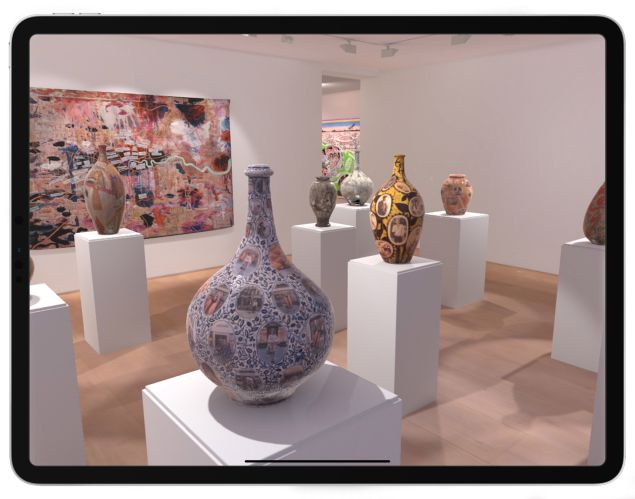
\includegraphics[width=6.36cm, height=5cm]{images/3d-gallery.jpg}
    \caption{AR Ausstellung - Beispiel}
    \label{fig:my_label}
\end{figure}

Das zentrale Element der Augmented Reality App ist eine Skulptur, die mit Hilfe von 3D-Objekterkennung erkannt wird und als Eingang in die virtuelle Welt dient.
Diese App bedient zwei User-Gruppen. Zum einen gibt es die User, die den Raum einrichten. Sie haben innerhalb der App Zugriff auf das Content-Management-System mit allen Assets der Studierenden und können diese frei im Raum platzieren und so die Austellung vorbereiten. Nachdem der Raum eingerichtet wurde, wird die Anordnung der Objekte gespeichert.

Die zweite User-Gruppe besteht aus den Besuchern. Sie nutzen die App, um sich alle Objekte anzuschauen. Der Raum sieht für alle Benutzer gleich aus und ermöglicht so ein Multi-User Erlebnis.

Um die Benutzererfahrung zu verbessern, werden die Lichtverhältnisse des Raum mit in die virtuelle Darstellung einberechnet, um eine realitätsnahe Visualisierung zu garantieren.

\subsection{Content-Management-System}

Die AR-App soll Zugriff auf die Assets der Studierenden bieten. Dazu zählen 3D-Objekte, Bilder, Videos, Audio-Dateien oder auch PDFs. Für eine einfache Verwaltung dieser Dateien muss ein Content-Management-System entwickelt werden.
Hier kann jeder Studierende seine auszustellenden Werke hochladen. Dazu wird zum einen ein Frontend für die Eingabe der Informationen benötigt und zum anderen ein Backend, welches die Dateien und Daten in einer Datenbank speichert.
Des Weiteren müssen API-Endpunkte erstellt werden, die die Kommunikation zwischen CMS und App herstellen.
Die korrekte Darstellung von 3D-Objekten muss gesichert werden, dies geschieht über eine Preview des Objekts schon während des Uploads, welches über Drittanbieter-Software (Sketchfab) gelöst wird.

\section{Zeitplan}
Das Projekt soll bis Ende September, bzw. Anfang Oktober beendet werden. Folgende Meilensteine sollen während des Arbeitsprozesses erreicht werden:
\begin{itemize}
    \item Erkennen des 3D-Objektes (Statue) mit mobilem Endgerät
    \item Platzieren von Bildern, Videos und 3D-Objekten im Raum (Kurator-Modus)
    \item Erstellen eines Content-Management-Systems
    \item Entwicklung einer CMS Backend-API
    \item Erstellen eines CMS Frontends
    \item Erstellen einer Sketchfab-Anbindung zum CMS um 3D-Objekte leichter zu speichern
    \item Streamen der Assets aus dem CMS in Unity
\end{itemize}
\section{Arbeitsteilung}
Die Arbeit am Projekt wird wie folgt aufgeteilt:
\begin{itemize}
    \item Marlon: Programmieren der Objekterkennung, Platzierung der 3D-Objekte
    \item Julius: Erstellen des CMS, Programmieren einer Backend API, Sketchfab Anbindung
    \item Vincent: Streamen der Daten aus dem CMS, Frontend-Entwicklung des CMS, Platzierung der 3D-Objekte
\end{itemize}
\section{Ressourcen}
Für die Umsetzung des Projektes benötigen wir Zugang zu drei iPad Pro mit LiDAR-Scannern. Um die Bilder, Videos, Audio-Dateien und 3D-Objekte zu sichern benötigen wir entsprechenden Webspace. Dieser kann kostengünstig bei Unternehmen wie Firebase von Google erworben werden oder wird von der HAW Hamburg selber gestellt. Die genaue Umsetzung sollte mit den Verantwortlichen diskutiert werden, um die für die HAW Hamburg beste Lösung zu finden.
\end{document}
